\chapter{Introduction}
\section{Context and motivation}
The rapid growth of cloud computing has led to a strong increase in the amount of data exchanged
inside modern datacenters. Services such as video and music streaming, cloud storage and online gaming 
already require large amounts of internal network bandwidth \todo[]{insert ref of 80\% of internet 
communication happens on intra-datacenter links}. More recently, the emergence of AI services such 
as ChatGPT, Gemini and Claude has accelerated this trend even further \todo{insert ref}. These applications rely on large clusters
of GPUs and servers that continually exchange data. As a result, 
the communication links between servers, switches and racks inside a datacenter are becoming an increasingly 
important bottleneck for these type of services.
\\
\\
To support this growth, datacenter interconnects are evolving towards 800~Gbit/s and 1.6~Tbit/s optical transceivers. 
These links are expected to play a key role in next-generation AI datacenters, where communication between accelerators and 
switching equipment must remain both high-speed and energy-efficient \cite{coherent_ecoc_2023}.
\\
\\
Today, most short-reach intra-datacenter optical links rely on \ac{IMDD}, 
often using \ac{PAM4} signalling. These techniques are relatively simple and power-efficient, which makes them 
attractive for short optical links. However, as symbol rates and transmission distances continue to increase,
\ac{IMDD} systems are reaching their limits in terms of chromatic dispersion tolerance, achievable spectral
efficiency and receiver sensitivity.

\begin{figure}[h]
\centering
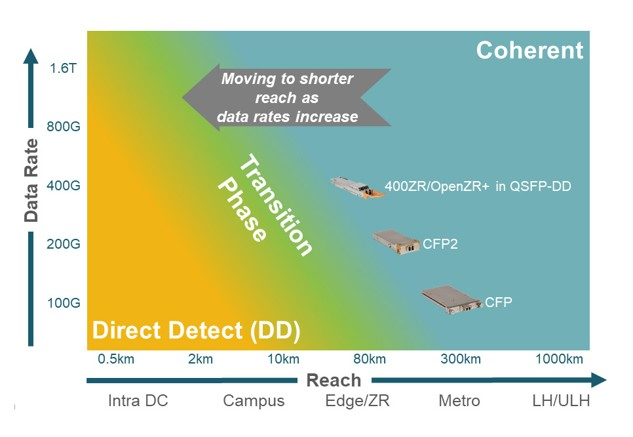
\includegraphics[width=0.7\linewidth]{figures/IMDD_versus_Coherent_Use.jpg}
\caption{This image needs to be referenced still.}
\label{fig:IMDD_versus_Coherent_Use}
\end{figure}
\todo{make more clear why this picture should be here}

Coherent optical communication offers an attractive alternative because it enables the use of higher-order 
modulation formats such as \ac{16QAM} while providing improved sensitivity and better tolerance to fiber impairments. 
Experimental comparisons between coherent and IMDD transceivers for intra-datacenter links have shown that coherent 
solutions can provide a larger optical power budget while maintaining comparable \ac{ASIC} power consumption 
\cite{Comparison_IMDD_Coherent_2019}.

\section{Problem statement}
Although coherent optical communication provides important advantages in terms of spectral efficiency and receiver 
sensitivity, these benefits come at the cost of increased receiver complexity. In particular, the \ac{DSP} chain of a coherent 
receiver contains computationally expensive blocks for frequency recovery and carrier phase recovery. 
\\\\
Carrier recovery is responsible for compensating the residual frequency offset and phase noise caused by the finite 
linewidth of the transmitter and local oscillator lasers. In conventional coherent receivers, this is often achieved 
through a combination of fourth-power frequency estimation and \ac{BPS}. The frequency recovery stage 
performs a coarse estimation of the carrier frequency offset, after which the phase recovery stage compensates the 
remaining phase rotation and phase noise.
\\
\\
However, both of these techniques become increasingly expensive as baudrates increase. Fourth-power frequency estimation 
typically relies on large FFT sizes in order to obtain sufficient frequency resolution. At the same time, blind phase 
search requires many test angles to achieve accurate phase estimation. This results in a significant amount of complex 
multiplications and memory usage, making carrier recovery one of the dominant contributors to the overall DSP complexity 
of a coherent receiver.\todo{source if applicable}
\\
\\
These complexity challenges are particularly important in intra-datacenter links, where power consumption and 
latency are critical constraints. In such environments, it is not sufficient for a carrier recovery algorithm to be 
accurate alone; it must also be implementable efficiently in hardware.
\\
\\
This thesis therefore investigates a low-complexity \ac{FPGA}-based carrier recovery architecture for baudrate-sampled 
16QAM coherent intra-datacenter links. The proposed approach aims to reduce the computational complexity of blind phase 
search while extending its effective frequency tracking range. This is achieved by combining a serialized blind phase 
search algorithm with an additional phase spread estimation block, allowing more robust carrier recovery with lower 
overall hardware cost.

\section{Objectives of this thesis}
A mathematical model of the proposed low-complexity carrier phase recovery system has 
already been developed in Simulink and will be discussed in more detail in Chapter
\ref{Proposed phase recovery architecture}. In this thesis, the implementation of this
phase recovery architecture on an \ac{FPGA} will be presented in detail. 

% Particular
% attention will be given to hardware-oriented optimizations that minimize both
% computational complexity and latency.

The proposed architecture forms the final stage of the receiver DSP chain, 
directly before the symbol decision stage. 

\begin{figure}[H]
\centering
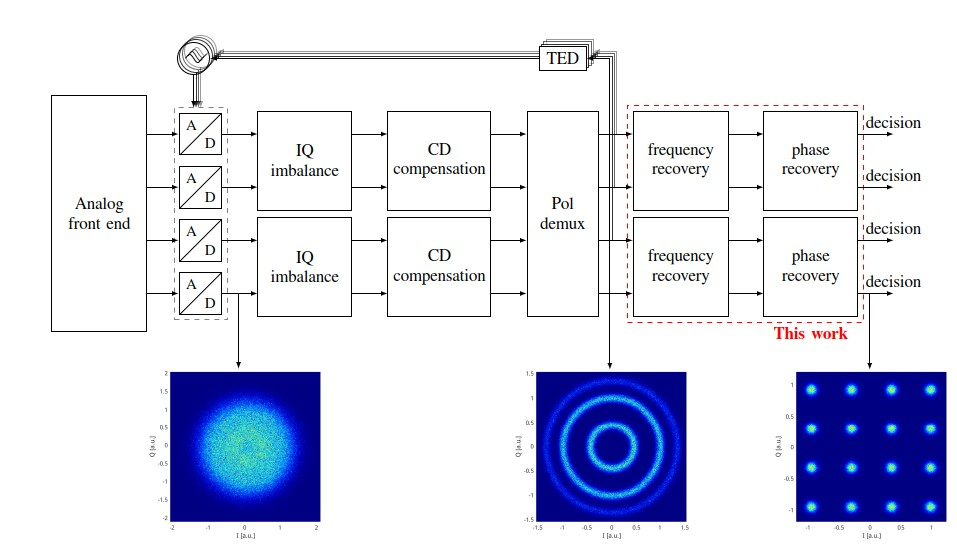
\includegraphics[width=0.9\linewidth]{figures/full-pipeline.jpg}
\caption{Full receiver DSP chain}
\label{fig:full-pipeline}
\end{figure}


Because of this position in the 
processing chain, its performance has a direct impact on the overall receiver 
quality. The implementation focuses not only on functional correctness,
but also on efficient hardware mapping, pipelining and memory usage.

Where multiple implementation strategies are possible, the motivation behind the
chosen design decisions will be discussed. Alternative approaches will also be
considered, together with the reasons why they were not selected in the final design.
\\\\
Finally, the performance of the implemented architecture will be evaluated. 
The proposed carrier recovery system contains several configurable parameters, 
such as the number of blind phase search stages, block size and phase-correction segments. 
Increasing these parameters can improve phase estimation accuracy and cycle slip 
tolerance, but also increases the required hardware resources, latency and power consumption.
\\\\
The objective of this evaluation is therefore not only to determine the absolute 
performance of the design, but also to investigate the trade-off between hardware 
cost and receiver performance under different operating conditions. These conditions 
include different signal-to-noise ratios, residual frequency offsets and laser linewidths, 
as these are the dominant impairments affecting coherent carrier recovery.


\section{Contributions}
\todo{keep this for after main body has been written}
This thesis presents the design and implementation of a low-complexity
phase spread estimation architecture for coherent communication systems.

The main contributions of this work are:

• A fixed-point hardware implementation of the spread estimation algorithm
  suitable for FPGA deployment.

• The design of a pipelined architecture for phase estimation,
  including dot-product, reciprocal multiplication, and arccos lookup blocks.

• The development of filtering techniques to improve estimation stability,
  including moving average filtering and sign majority voting.

• A verification framework using Python reference models and VHDL
  testbenches to validate the fixed-point implementation.

• A performance evaluation of the proposed architecture in terms of
  numerical accuracy, latency, and resource usage.
  
\section{Thesis outline}
The remainder of this thesis is structured as follows:
\\\\
Chapter \ref{Background} introduces the theoretical background 
required for this work. First, coherent optical communication 
systems are discussed, with a focus on how phase noise and residual 
frequency offset arise in these systems and how they affect the 
received signal. This is necessary to understand why carrier recovery 
is required and what challenges it introduces. Next, existing carrier 
recovery techniques are reviewed, together with their limitations and 
motivation for the proposed approach. The digital representation of 
\ac{16QAM} signals is then discussed, since the proposed architecture 
strongly depends on fixed-point symbol scaling, numerical precision 
and \ac{SNR}-related considerations. Finally, a section is dedicated 
to the \ac{CORDIC} algorithm. Unlike the other algorithmic blocks in 
this thesis, which are developed specifically for this work, the 
\ac{CORDIC} is based on an existing \ac{IP} core developed by 
[INSERT REF]\todo{insert ref CORDIC IP}.
\\\\
Chapter \ref{Proposed phase recovery architecture} presents the proposed phase recovery 
algorithm from a theoretical perspective. Building on the concepts introduced in the previous 
chapter, the complete architecture is divided into its main functional blocks, including the 
\ac{SBPS}, \ac{SE}, \ac{PU} and \ac{PC} modules. For each subblock, the operating 
principle, mathematical model and expected contribution to the overall system are discussed. 
The theoretical performance of the proposed method is also analysed, based on the work of 
J. De Busscher in [INSERT REF]\todo{insert ref PAPER JONAS}. 

% \todo{redo}Particular attention is given to 
% how the proposed spread estimation extends the frequency tracking range of the phase recovery 
% system while maintaining a low computational complexity.

Chapter \ref{Hardware Implementation} describes how the theoretical carrier recovery system is 
translated into an \ac{FPGA} implementation. This chapter discusses the practical challenges 
associated with such an implementation, including fixed-point numerical representations, 
timing closure, and hierarchical design. In addition, it explains how the individual
subblocks are combined into a complete processing chain and how dataflow, valid signals and latency 
alignment are handled throughout the design. 
\\\\
Chapter \ref{Verification and simulation} explains the simulation and verification framework used for 
the implemented design. The testbenches of the different subblocks are discussed together with their 
corresponding results. The purpose of this chapter is to show that the hardware implementation behaves 
in accordance with the theoretical model and to explain any deviations between both. The focus is 
therefore on functional correctness rather than on overall system performance under different operating 
conditions. Comparisons between the \ac{FPGA} implementation and the Python or Simulink reference models 
are also included to demonstrate that the implemented fixed-point design accurately reproduces the 
expected behaviour.
\\\\
Chapter \ref{Results} evaluates the overall performance of the implemented carrier recovery system. 
Separate sections discuss the performance of the \ac{SBPS} and \ac{SE} blocks and identify the 
conditions under which their performance begins to degrade. The influence of different system 
parameters, such as block size, number of search stages and datapath-bitlengths, is also investigated. In addition, this chapter discusses the hardware 
resource usage and latency of the final design. The relation between 
implementation complexity and system performance is analysed in order to determine which parameters 
offer the most favourable trade-off.

% Finally, Section \ref{Comparison with reference method} compares 
% the proposed implementation with currently used reference methods and highlights the advantages of the 
% proposed architecture in terms of cycle slip tolerance, frequency tracking range and computational 
% efficiency.

Chapter \ref{Discussion} discusses the limitations of the current implementation and identifies 
possible improvements for future work. This includes both algorithmic improvements and hardware-related 
optimizations. Potential extensions such as more advanced \ac{LUT} implementations, adaptive parameter 
selection, improved spread estimation for low \ac{SNR} conditions and support for higher-order 
modulation formats are considered\todo{find good alternative solutions, these are purely speculative}. 
In addition, the discussion reflects on the assumptions made 
throughout the work, such as the assumption that the residual frequency 
offset changes only slowly between neighbouring blocks. The chapter also provides a broader overview 
of the main design trade-offs and explains how these trade-offs influenced the final architecture.
\\\\
Finally, Chapter \ref{Conclusion} summarizes the most important aspects of the work. 
It revisits the original objectives of the thesis, discusses the extent to which these objectives were 
achieved and reflects on the main findings of the implementation and evaluation. The final chapter also 
outlines possible directions for future work, including integration into a complete coherent receiver 
chain and further optimization of the architecture for practical deployment.